%%=============================================================================
%% Methodologie
%%=============================================================================

\chapter{\IfLanguageName{dutch}{Methodologie}{Methodology}}
\label{ch:methodologie}

%% TODO: Hoe ben je te werk gegaan? Verdeel je onderzoek in grote fasen, en
%% licht in elke fase toe welke stappen je gevolgd hebt. Verantwoord waarom je
%% op deze manier te werk gegaan bent. Je moet kunnen aantonen dat je de best
%% mogelijke manier toegepast hebt om een antwoord te vinden op de
%% onderzoeksvraag.

In dit hoofdstuk zal er dieper ingegaan worden op het onderzoek van deze bachelorproef. De verschillende parsers die binnen dit onderzoek worden gebruikt zijn reeds toegelicht in de Stand van Zaken \ref{ch:stand-van-zaken}. Dit hoofdstuk gaat hun implementatie verder toelichten in de context van deze bachelorproef. De eerste twee secties gaan dieper in op de start van het onderzoek, hoe het onderzoek is opgesteld, de basis van het onderzoek, de gekozen technologie en de verschillende testen die zullen worden uitgevoerd. Hierna volgen er verschillende secties die dieper ingaan op hoe het onderzoek is uitgevoerd en op welke manier de code is opgebouwd, aangepast, etc..


\section{Opzetting van het onderzoek}
Omdat dit onderzoek gebaseerd is op een reeds uitgebrachte paper is het zinvol om eerst te kijken naar het voorgaande onderzoek. De paper waarop deze bachelorproef gebaseerd is, `Tools and Benchmarks for Automated Log Parsing` \autocite{TBA2019}, heeft tezamen met een andere paper `An Evaluation Study on Log Parsing and Its Use in Log Mining` \autocite{he2016evaluation} reeds een opensource repository op GitHub staan met alle code voor de parsers binnen deze papers \footnote{https://github.com/logpai/logparser}. Hierbij zat een documentatie \footnote{https://logparser.readthedocs.io/} die uitleg gaf over hoe de repository moest gedownload en geïnstalleerd worden en hoe de tool gebruikt kon worden.\\

De log parsers die niet tot deze paper behoren hebben elk een duidelijke paper waarin de algoritmes toegelicht worden alsook GitHub repositories \footnote{NuLog repository: https://github.com/nulog/nulog} \footnote{Logram repository: https://github.com/BlueLionLogram/Logram} van de makers waarin reeds een implementatie verwerkt staat. Deze parsers zullen dus op een gelijkaardige manier moeten ingewerkt worden in de Benchmark tool zodat deze op dezelfde manier getest kunnen worden en er dus een duidelijke vergelijking kan gemaakt worden.\\

In de onderstaande subsecties worden twee delen van de opzetting van het onderzoek besproken. De technologie sectie bevat de verschillende technologieën die nodig zijn om dit onderzoek uit te voeren en hoe deze moeten worden opgezet en de vergelijkingscriteria subsectie bevat een oplijsting van de verschillende criteria waarop er zal gelet worden tijdens de vergelijking van de verschillende log parsers.

\subsection{Technologie}
\label{section:Technologie}
Een groot deel van de opzetting van de technologie binnen dit onderzoek wordt reeds behandeld in de documentatie van de repository van de paper `Tools and Benchmarks for Automated Log Parsing` \autocite{TBA2019} \footnote{https://logparser.readthedocs.io/}.\\

Hieronder valt ten eerste de opzetting met Docker. Docker is een manier de volledige repository met alle benodigdheden te installeren als een container op de gekozen computer. Dit wordt vooral gebruikt binnen Linux en daarom wordt er ook aangeraden om op een Linux machine te werken. Binnen dit onderzoek is er echter gewerkt met een Windows machine omdat deze parsers op elke machine zouden moeten werken en zo geeft dit onderzoek ook een weergave voor de opzet met Windows. Om Docker te gebruiken op Windows moet eerst de Docker desktop applicatie gedownload worden. Deze implementatie was echter niet eenvoudig en voor dit onderzoek is er na het proberen van Docker desktop gekozen om toch op de conventionele manier te werken vanaf de GitHub repository.\\

Na het clonen van de repository zou alles klaar moeten zijn om deze logparser repository te gebruiken. De repositories van de andere log parsers zijn overgenomen vanuit GitHub en toegevoegd aan de logpai repository. Dit heeft als resultaat dat binnen deze bachelorproef ook één grote testomgeving aanwezig is en deze zal aanwezig zijn op de GitHub repository \footnote{https://github.com/MarbodNaassens/Bachelorproef\_HOGENT} van deze bachelorproef.

Om deze repository te gebruiken is het belangrijk om te weten wat de machine specificaties waren binnen dit onderzoek. Deze staan hieronder weergegeven:
\begin{itemize}
    \item OS: Windows 10 Home v20H2 (64-bit)
    \item CPU: Intel(R) Core(TM) i5-7300HQ CPU @ 2.50GHz
    \item RAM: 16GB
    \item Python version: 3.9.5
\end{itemize}

Omdat er gewerkt wordt met de GitHub repository in plaats van Docker moeten hiernaast nog python libraries toegevoegd worden zoals: hashlib, keras, math, pandas, regex, scikit-learn, sys, tensorflow, torch en tqdm. Deze kunnen allemaal geïmplementeerd worden door:
\begin{verbatim}
    pip install <library>
\end{verbatim}
Bij het Python verhaal komen ook nog aanpassingen aan de code kijken en deze aanpassingen worden verder toegelicht in sectie \ref{section:testen}.

Bij het onderzoek is wel gebleken dat de parser `SLCT` niet op Windows kan gebruikt worden. Deze werkt namelijk met C code maar zelfs met de juiste GCC compiler, i.e.\ dit is een compiler nodig voor het runnen van C code, geeft deze parser geen resultaten. Voor deze parser te testen is er gewerkt geweest met een virtuele machine met de volgende specificaties:
\begin{itemize}
    \item OS: Fedora v34 (64-bit)
    \item RAM: 4GB
\end{itemize}

Voor deze opzet werd Oracle VirtualBox \footnote{https://www.virtualbox.org/} gebruikt tesamen met een Fedora iso afbeelding \footnote{De x86\_64 iso op https://getfedora.org/en/workstation/download/}, i.e.\ een container die wordt gebruikt om virtueel fedora te kunnen gebruiken. Deze versie van fedora bezit reeds een GCC compiler om SLCT te kunnen runnen. Hiernaast werd de hierboven vermelde opzetting van de logpai repository toegepast. Python 3 moest natuurlijk wel nog geïnstalleerd worden tesamen met de benodigde libraries. Voor de installatie van Python 3.8.7 op Linux werd de volgende code gebruikt:
\begin{verbatim}
    sudo yum install gcc openssl-devel bzip2-devel libffi-devel
    cd /opt
    wget https://www.python.org/ftp/python/3.8.7/Python-3.8.7.tgz
    tar xzf Python-3.8.7.tgz
    cd Python-3.8.7
    sudo ./configure --enable-optimizations
    sudo make altinstall
    sudo rm Python-3.8.7.tgz
    python3.8 -V
\end{verbatim}

Hiernaast moesten ook nog dezelfde aanpassingen aan de python code gebeuren zoals verder zal uitegelgd worden in sectie \ref{section:testen}. Deze aanpassingen moesten hierbij uitgevoerd door het volgend commando te runnen:
\begin{verbatim}
    gedit /logparser/logparser/<folder>/<file>
\end{verbatim}

Dit was nodig omdat de gedownloadde files onder `read-only` access stonden. Om dit commando uit te voeren moet er wel als de root user aangemeld worden.


De opbouw van dit onderzoek zal te vinden zijn in de repository van deze bachelorproef onder de map `BP\_onderzoek`. Deze map bevat verschillende files en folders. Hieronder zal een toelichting gegeven worden over de inhoud van deze folders:
\begin{itemize}
    \item LogParse: Deze folder bevat het onderzoek in verband met LogParse. Hierin zal de implementatie van de gekozen parsers aanwezig zijn voor het testen van een online omgeving. Om deze code te kunnen laten lopen moet er vanuit deze folder gewerkt worden. Verdere implementatie wordt besproken in de sectie \ref{subsection:OnlineOffline}.\\
    
    \item Parsers: Deze folder zal in het onderzoek alle implementaties van de logparsers bevatten. Deze implementaties zijn geschreven in Python omdat dit de taal is die gekozen is door de vorige paper en algemeen bekend staat als een goede taal voor data verwerking. Ook zal het makkelijker zijn om de parser `NuLog` te implementeren via Python omdat deze reeds een library bevat voor het werken met Neurale Netwerken en NLP.\\
    
    \item Service: Deze folder zal in het onderzoek alle test bestanden bevatten die gebruikt worden om de log bestanden door de parser te laten verwerken en om vergelijkende waarden terug te krijgen. Ook zullen de resultaten van vorige onderzoeken hierin teruggevonden worden. Om de test bestanden te laten lopen zal er moeten gewerkt worden in de command line vanaf deze folder. Bijvoorbeeld zo zal voor Drain het volgend commando uitgevoerd moeten worden:
    
    \begin{verbatim}
        python3 ./Drain_benchmark.py
    \end{verbatim}

    \item Logs: Deze folder zal in het onderzoek alle log bestanden bevatten, i.e.\ tekst bestanden met daarin onverwerkte log messages. Hiernaast zal deze ook de verwachtte gestructureerde uitkomsten en clusters bevatten.
\end{itemize}

\subsection{Vergelijkingscriteria}
Het is niet eenvoudig om log parsers te vergelijken omdat hun werking zeer verschillend is en het niet realistisch is om elke parsing van elke lijn te gaan analyseren. Daarom moeten er duidelijke criteria worden opgesteld waarmee deze parsers zullen vergeleken worden. Op basis van deze criteria zal een antwoord op de onderzoeksvraag gezocht worden. Hieronder zal een overzicht gegeven worden van de verschillende criteria:
\begin{itemize}
    \item Tijd: Tijd is een factor die een grote rol zal spelen omdat er gezocht wordt naar een parser die in real-time snel logs kan verwerken. Dit criterium zal gemeten worden aan de hand van een timer.
    
    \item Manuele check: Een manuele check zal uitgevoerd worden op de eerste 20 lijnen van een log cluster uitkomst om te zien of deze parsing wel zinvol is en geen te specifieke of te generieke waarden doorgeeft. Er zal gekeken worden naar het aantal clusters dat gegenereerd wordt tijdens de parsing, \lq Is dit een groot/klein aantal? Is dit aantal te groot (specialisatie) of te klein (generalisatie)?\rq. Alsook zal er gekeken worden naar de clusters zelf of deze wel nuttig zijn en duidelijke patronen weergeven. Dit is een belangrijk gegeven om zeker te zijn dat er geen underfitting of overfitting ontstaat tijdens de parsing.\\
    
    \item F-Score: De F-score is een gekende maatstaf in de statistiek. Dit is een formule die gebruikt wordt om de accuraatheid van een bepaalde test te berekenen. Hoe dichter deze score bij 1 neigt hoe beter de accuraatheid van de test. Deze score wordt berekend door de precisie en recall van een test. Binnen dit onderzoek wordt de precisie berekend door de volgende formule: 
    
    \[\frac{\text{\# gevonden patronen die tot de oplossing behoren}}{\text{Totaal \# gevonden patronen}}\]
    
    en de recall wordt berekend door de formule: 
    
    \[\frac{\text{\# gevonden patronen die tot de oplossing behoren}}{\text{Totaal \# patronen in de oplossing}}\]
    
    Hierbij hangt de waarde van het gevonden aantal patronen die tot de oplossing behoren ook af van het aantal keer dat deze voorkomen. Dit aantal moet gelijk zijn aan het aantal in de oplossing.\\
    
    \item Accuraatheid: De accuraatheid slaat op het aantal patronen die de parser succesvol heeft kunnen achterhalen losstaand van het aantal keer dat deze voorkomt binnen de oplossing. Hierbij wordt de volgende formule berekend: \[\frac{\text{Totaal \# correct geparste log messages}}{\text{Totaal \# log messages in de oplossing}}\] Een log message wordt beschouwd als correct geparsed als deze in dezelfde groep zit met dezelfde log messages als in het verwachte gestructureerde voorbeeld. Bijvoorbeeld als een log message $A$ een groep deelt met twee andere $B$ en $C$, maar de parser zet $A$ in een groep met twee log messages $D$ en $E$ dan zal de accuraatheid maar $\frac{1}{3}$ zijn.\\
    
   \item Online vs. Offline: Er zal ook gekeken worden hoe de parsers met de beste uitkomsten als online methodes kunnen omgaan met nieuwe data en deze uitkomsten zullen vergeleken worden met die van het offline verwerken. Hiervoor zal LogParse gebruikt worden omdat deze implementatie aan de hand van een training en test set het toekomen van nieuwe logs kan nabootsen.
\end{itemize}

\section{Testen van benchmarks}
\label{section:testen}
Bij het testen van de verschillende parsers wordt er gebruik gemaakt van de verschillende vergelijkingscriteria. Deze criteria zijn het makkelijkst op te lijsten in een tabel zodat er een mooi overzicht is voor de vergelijking van deze parsers en dit zal weergegeven worden in de laatste sectie van deze sectie waarbij alle parsers, de reeds onderzochte en de nieuwe, zullen opgelijst worden.\\

De parsers die zich in de reeds vernoemde paper bevinden waren makkelijk te testen omdat de code hiervoor reeds geoptimaliseerd was. Er moesten echter wel een paar aanpassingen gebeuren omdat dit onderzoek werd uitgevoerd met een oudere versie van Python. Het is aan te raden om altijd mee te zijn met de nieuwste versie van de technologie dus werd dit onderzoek uitgevoerd met Python 3.9.5. De versie van de vorige paper was Python 2.7 dit betekende dat er aanpassingen moesten gebeuren aan imports en er methodes moesten aangepast worden omdat ze `deprecated`, i.e.\ niet meer gesupporteerd, waren. De aanpassingen worden hieronder weergegeven:
\begin{itemize}
    \item Regex: In de verschillende parser files wordt er gebruik gemaakt van $re$ voor reguliere expressies te verwerken en dit wordt geïmporteerd aan de hand van de code: 
    \begin{verbatim}
        import re
    \end{verbatim}
    Dit werkt echter niet meer in Python 3 dus dit moet aangepast worden naar:
    \begin{verbatim}
        import regex as re
    \end{verbatim}

    \item Scipy: Gelijkaardig aan het vorige punt is `scipy.misc` niet meer een geldige import en moet deze import in evaluator.py (binnen de utils folder), utils.py (binnen de scikit-extremes/sk-extremes folder) en wind.py (binnen de scikit-extremes/sk-extremes/models folder) aangepast worden naar het volgende:
    \begin{verbatim}
        from scipy.special import *
    \end{verbatim}

    \item Dictionary iteratie: Om over dictionaries te itereren werd in Python 2.7 $.iteritems$ gebruikt maar binnen Python 3 is dit vervangen door $.items$. Dit moest aangepast worden in alle benchmark bestanden. Hiernaast moest dit aangepast worden in de volgende bestanden: MoLFI.py, LogSig.py, regexmatch.py, RI\_precision.py (binnen de LogParse folder), logTIM.py (binnen de LogParse folder), classifier.py (binnen de LogParse folder), checkVocab.py (binnen de LogParse folder).\\
    
    \item Folders: Naast deze aanpassingen werd binnen deze bachelorproef een eigen folder structuur opgesteld en hiervoor moesten bepaalde imports aangepast worden. Zo moesten in de $\_\_init\_\_.py$ bestanden van de parsers de imports aangepast worden door een punt voor de naam van de parser te zetten, bijvoorbeeld:
    \begin{verbatim}
        from .Drain import *
    \end{verbatim}
\end{itemize}

Naast het aanpassen van de code door de verandering naar de nieuwste Python versie is testen geen probleem. Een uitzondering hierop is de parser SLCT omdat deze parser deels in C is geschreven. Om de C code te kunnen runnen moet er gezorgd worden dat er een versie van GCC beschikbaar was op de computer en zelfs na de installatie werkt deze parser niet naar behoren op een Windows machine. Om dit op te lossen wordt aangeraden om Linux te gebruiken zoals reeds vermeld in de vorige sectie \ref{section:Technologie}\\

\section{Toevoegen en testen van nieuwe parsers}
Voor het toevoegen van de nieuwe parsers aan deze reeds bestaande tool moesten er meer aanpassingen gebeuren dan enkel het versiebeheer. Hieronder zal er een duidelijke weergave gegeven worden van de verschillende extra log parsers en hun inwerking in de benchmarking tool:
\begin{itemize}
    \item Logram: Logram was een moeilijke parser om in te werken in de tool. Er was reeds een github repository die open werd gesteld door de schrijver van de paper, `Logram: Efficient Log Parsing Using n-Gram Dictionaries` \autocite{dai2020logram}. De code was wel reeds gebaseerd op dezelfde logs en aldus makkelijk te testen vanaf dat deze geïmplementeerd was maar er waren verschillen bij zoals dat er gewerkt werd met Apache Spark. Hierbij moest dus een versie van Apache Spark aanwezig zijn om deze te kunnen runnen. Dit omdat verscheidene functies binnen de code op deze import rekenen. Voor dit onderzoek is er gebruik gemaakt van versie 3.1.1 van Spark. \\
    
    Een ander duidelijk verschil is dat er van deze parser reeds verschillende versies beschikbaar waren, i.e.\ een online en offline versie. Hierbij werd binnen dit onderzoek naar de online versie gekeken omdat deze het interessantst is voor dit onderzoek.\\
    
    De folder structuur van de repository is behouden zodat de code geen problemen zou geven en daarom wordt deze parser onder de folder `parsers` uitgevoerd. Bij het testen van deze parser moeten er twee bestanden uitgevoerd worden, enerzijds het bestand $Main.py$ binnen de folder `LogAbstractionOL` en anderzijds het bestand $Main.py$ binnen de folder `Evaluation`. In deze laatste folder worden per dataset de bijhorende parameters weergegeven voor de thresholds die automatisch berekend zijn voor de 2-grams en 3-grams respectievelijk.\\
    
    \item NuLog: NuLog was makkelijker in te werken in de tool omdat de code gebaseerd was op de tool en dezelfde benchmarks gebruikte. Hierbij moesten er eerst en vooral aanpassingen gebeuren voor de werking met Python 3.9 en voor de implementatie van neurale netwerken (zoals het installeren van scikit learn). Na deze aanpassingen was de parser makkelijk te testen maar het testen van deze parser nam wel veel tijd in beslag. Bij het uitvoeren van deze parser wordt steeds een nieuw model opgesteld voor elke dataset waardoor dit veel vermogen vraagt van een CPU en aldus een substantieel aantal tijd in neemt. Hierbij moet ook vermeld worden dat nog niet elke dataset ingewerkt was binnen NuLog dit betekende dat binnen dit onderzoek deze overige zelf ingewerkt moeten worden
    
    \item LogParse: LogParse heeft het voordeel dat het reeds getest was met dezelfde parsers en log bestanden als in de paper `Tools and Benchmarks for Automated Log Parsing` \autocite{TBA2019}. Hierbij was de moeilijkheidsgraad eerder het structureren en vinden van de juiste files om deze samen te voegen omdat op de Github repository \footnote{https://github.com/NetManAIOps/LogParse} de parser files niet altijd bij elkaar staan. Buiten dit structureren zal het inwerken van eventuele nieuwe parsers problematisch kunnen zijn door de structuur.
\end{itemize}

\section{Vergelijkende studie van de verschillende parsers}
Deze sectie bevat de weergaves van de vergelijkingen tussen de verschillende parsers. Door te kijken naar de verschillende vergelijkingscriteria die werden besproken in de vorige secties kunnen er duidelijke tabellen opgesteld worden met de waarden die elke log parser behaalt op de verschillende data sets. In de tabellen zal het `Offline vs Online` principe niet aangehaald worden.\\

Het Offline vs Online principe wordt toegelicht in de laatste sectie \ref{subsection:OnlineOffline} waarbij er dieper wordt ingegaan op LogParse en het online testen van de gekozen parsing methodes. Het online principe is deel van de onderzoeksvraag en daarom wordt dit apart aangehaald.\\

\subsection{Vergelijkingstabellen}
De vergelijkende tabellen die hieronder weergegeven worden zijn tabellen die de prestaties van de parsers weergeven op de fractionele datasets, i.e.\ de datasets die beperkt zijn tot de eerste 2000 lijnen van een log file.

Deze tabellen op zich zeggen al redelijk veel over de performantie van de parsers. In de tabellen zijn de grootste waarden van elke kolom vet gedrukt. Dit geeft een makkelijker overzicht over de waarden. Bij het aantal clusters wordt de waarde die het dichtst bij de verwachte waarde ligt vet gedrukt. Hiernaast worden ook in de parser kolom de drie beste parsers vet gedrukt om zo een overzicht te houden voor het latere onderzoek waar we eventuele offline parsers online kunnen laten opereren. Deze parsers zullen worden gekozen door eerst en vooral te kijken naar de accuraatheid, hiernaast naar de tijd en de f-score en uiteindelijk naar het aantal clusters. Hierdoor kunnen sommige parsers die niet de hoogste waarde binnen een bepaalde kolom bezitten ook gekozen worden als ze de tweede hoogste waarde bezitten.\\

Er wordt vooral naar de accuraatheid en snelheid gekeken omdat deze twee de belangrijkste waarden zijn voor het antwoord op deze bachelorproef. Een parser die snel werkt maar niet accuraat is of een parser die traag werkt maar een goede accuraatheid levert, is niet interessant.

Wat ook belangrijk is om te weten is dat sommige waarden als niet aanwezig (N/A) worden geschouwd. Deze waarden zullen hieronder toegelicht worden:
\begin{itemize}
    \item LogCluster : Bij LogCluster wordt het aantal clusters weggelaten. Dit is omdat bij het onderzoek deze niet automatisch achterhaald konden worden.\\
    
    \item NuLog: Bij NuLog worden twee kolommen leeggelaten. Ten eerste wordt het aantal clusters weggelaten en dit is omdat de implementatie van NuLog geen clusters weergaf waardoor dit giswerk zou geweest zijn. De accuraatheid geeft hier echter een terugval op. Ten tweede word de tijd weggelaten omdat deze parser begint met het opstellen van een model en dit een grote hoeveelheid tijd inneemt maar dit model moet wel maar één keer opgesteld worden in het begin dus dit is geen goeie representatie voor deze parser.
    
    \item IPLoM: Zoals in tabel \ref{table:Mac} te zien is staan alle waarden voor deze parser op `N/A`. Dit is omdat deze parser binnen dit onderzoek altijd vastliep bij contact met deze dataset.
\end{itemize}

In deze tabellen wordt een vergelijkingscriterium niet vermeld en dat is het `Manuele check` criterium. Deze wordt in de volgende sectie verder toegelicht. Deze manuele observatie zal verder bouwen op de resultaten gegeven in de tabellen. De resultaten zullen dan ook binnen deze sectie besproken worden.

\begin{table}[!hbtp]
    \caption{Tabel met vergelijking van alle log parsers met toepassing op de fractionele data set Android.}
    \label{table:Android}
    \begin{center}
        \begin{tabular}{||c | c | c | c | c||} 
            \hline
            Parser & Tijd & F-Score & Accuraatheid & Aantal clusters \\ [0.5ex] 
            \hline\hline
            SLCT & 2.70s & 0.9837 & 0.8815 & 179 \\
            
            AEL & 0.28s & 0.9404 & 0.6815 & 148 \\ 
            
            IPLoM & 0.32s & 0.9662 & 0.7795 & 158 \\
            
            LKE & 95.22s & 0.9921 & 0.9085 & 189 \\
            
            LFA & 0.26s & 0.0786 & 0.0000 & 154 \\
            
            LogSig & 88s & 0.8441 & 0.5325 & 172 \\
            
            SHISO & 4.53s & 0.8437 & 0.5850 & 171 \\
            
            LogCluster & 0.45s & 0.9840 & 0.7975 & N/A \\
            
            \textbf{LenMa} & 0.78s & 0.9922 & 0.8795 & \textbf{161} \\
            
            LogMine & 3.98s & 0.8934 & 0.5040 & 116 \\
            
            \textbf{Spell} & 0.56s & 0.9922 & \textbf{0.9185} & 180 \\
            
            \textbf{Drain} & 0.43s & \textbf{0.9959} & 0.9110 & 171 \\
            
            MoLFI & 16s & 0.8589 & 0.6675 & 144 \\
            
            Logram & \textbf{0.13s} & 0.9750 & 0.7945 & 113 \\
            
            NuLog & N/A & 0.9727 & 0.8225 & N/A \\
            \hline
        \end{tabular}
    \end{center}
\end{table}


\begin{table}[!hbtp]
    \caption{Tabel met vergelijking van alle log parsers met toepassing op de fractionele data set Apache.}
    \label{table:Apache}
    \begin{center}
        \begin{tabular}{||c | c | c | c | c||} 
            \hline
            Parser & Tijd & F-Score & Accuraatheid & Aantal clusters \\ [0.5ex] 
            \hline\hline
            SLCT & 2.14s & 0.9429 & 0.7305 & 10 \\
            
            \textbf{AEL} & \textbf{0.18s} & \textbf{1.0000} & \textbf{1.0000} & \textbf{6} \\ 
            
            \textbf{IPLoM} & 0.25s & \textbf{1.0000} & \textbf{1.0000} & \textbf{6}  \\
            
            LKE & 112.87s & \textbf{1.0000} & \textbf{1.0000} & \textbf{6}  \\
            
            LFA & 0.20s & 0.4943 & 0.0000 & \textbf{6}  \\
            
            LogSig & 0.94s & 0.9498 & 0.7305 & 7 \\
            
            SHISO & 0.77s & \textbf{1.0000} & \textbf{1.0000} & \textbf{6}  \\
            
            LogCluster & 0.49s & 0.9424 & 0.7085 & N/A \\
            
            LenMa & 0.55s & \textbf{1.0000} & \textbf{1.0000} & \textbf{6}  \\
            
            LogMine & 1.85s & \textbf{1.0000} & \textbf{1.0000} & \textbf{6} \\
            
            Spell & 0.35s & \textbf{1.0000} & \textbf{1.0000} & \textbf{6}  \\
            
            \textbf{Drain} & 0.32s & \textbf{1.0000} & \textbf{1.0000} & \textbf{6} \\
            
            MoLFI & 1.18s & \textbf{1.0000} & \textbf{1.0000} & \textbf{6} \\
            
            Logram & 0.20s & 0.6377 & 0.3125 & 16 \\
            
            NuLog & N/A & \textbf{1.0000} & \textbf{1.0000} & \textbf{6} \\
            \hline
        \end{tabular}
    \end{center}
\end{table}


\begin{table}[!htp]
    \caption{Tabel met vergelijking van alle log parsers met toepassing op de fractionele data set BGL.}
    \label{table:BGL}
    \begin{center}
        \begin{tabular}{||c | c | c | c | c||} 
            \hline
            Parser & Tijd & F-Score & Accuraatheid & Aantal clusters \\ [0.5ex] 
            \hline\hline
            SLCT & 1.89s & 0.9552 & 0.5725 & 79 \\
            
            AEL & 0.22s & 0.9996 & 0.9570 & 107 \\ 
            
            IPLoM & 0.38s & 0.9991 & 0.9390 & 106 \\
            
            LKE & 179.86s & 0.3994 & 0.1275 & 190 \\
            
            LFA & 0.23s & 0.2671 & 0.0000 & 104 \\
            
            LogSig & 136.70s & 0.9332 & 0.2320 & 128 \\
            
            SHISO & 5.59s & 0.9944 & 0.7110 & 155 \\
            
            LogCluster & 0.50s & 0.9970 & 0.8350 & N/A \\
            
            LenMa & 3.06s & 0.9394 & 0.6895 & 317 \\
            
            LogMine & 0.37s & 0.9700 & 0.7245 & 49 \\
            
            Spell & 0.64s & 0.9569 & 0.7865 & 262 \\
            
            \textbf{Drain} & 0.44s & 0.9996 & 0.9625 & 108 \\
            
            MoLFI & 14.16s & 0.9993 & 0.9500 & 136 \\
            
            \textbf{Logram} & \textbf{0.13s} & 0.9560 & 0.5870 & \textbf{122} \\
            
            \textbf{NuLog} & N/A & \textbf{0.9997} & \textbf{0.9710} & N/A \\
            \hline
        \end{tabular}
    \end{center}
\end{table}


\begin{table}[!htp]
    \caption{Tabel met vergelijking van alle log parsers met toepassing op de fractionele data set Hadoop.}
    \label{table:Hadoop}
    \begin{center}
        \begin{tabular}{||c | c | c | c | c||} 
            \hline
            Parser & Tijd & F-Score & Accuraatheid & Aantal clusters \\ [0.5ex] 
            \hline\hline
            SLCT & 1.30s & 0.8112 & 0.4220 & 13 \\
            
            AEL & 0.23s & 0.9959 & 0.8690 & 131 \\ 
            
            \textbf{IPLoM} & 0.37s & 0.9964 & \textbf{0.9540} & 97 \\
            
            LKE & 111.94s & 0.2205 & 0.0000 & 1 \\
            
            LFA & 0.22s & 0.2205 & 0.0000 & 103 \\
            
            LogSig & 7.77s & 0.9913 & 0.6325 & 23 \\
            
            \textbf{SHISO} & 8.28s & 0.9975 & 0.8670 & \textbf{112} \\
            
            LogCluster & 0.46s & 0.8856 & 0.5630 & N/A \\
            
            LenMa & 0.98s & 0.9965 & 0.8850 & 151 \\
            
            LogMine & 4.19s & 0.9955 & 0.8695 & 127 \\
            
            Spell & 0.56s & 0.9202 & 0.7775 & 167 \\
            
            \textbf{Drain} & 0.38s & \textbf{0.9990} & 0.9200 & 103\\
            
            MoLFI & 18.12s & 0.9968 & 0.8910 & 178 \\
            
            Logram & \textbf{0.14s} & 0.7825 & 0.4510 & 104 \\
            
            NuLog & N/A & 0.9152 & 0.5495 & N/A \\
            \hline
        \end{tabular}
    \end{center}
\end{table}


\begin{table}[!htp]
    \caption{Tabel met vergelijking van alle log parsers met toepassing op de fractionele data set HDFS.}
    \label{table:HDFS}
    \begin{center}
        \begin{tabular}{||c | c | c | c | c||} 
            \hline
            Parser & Tijd & F-Score & Accuraatheid & Aantal clusters \\ [0.5ex] 
            \hline\hline
            SLCT & 1.24s & 0.9658 & 0.5450 & 11 \\
            
            \textbf{AEL} & 0.22s & \textbf{1.0000} & 0.9975 & 16 \\ 
            
            \textbf{IPLoM} & 0.33s & \textbf{1.0000} & \textbf{1.0000} & \textbf{14} \\
            
            LKE & 63.30s & \textbf{1.0000} & \textbf{1.0000} & \textbf{14}  \\
            
            LFA & 0.28s & 0.2261 & 0.0000 & 15 \\
            
            LogSig & 1.69s & 0.8784 & 0.5080 & 13 \\
            
            SHISO & 1.43s & \textbf{1.0000} & 0.9975 & 16 \\
            
            LogCluster & 0.41s & 0.9519 & 0.5460 & N/A \\
            
            LenMa & 0.61s & \textbf{1.0000} & 0.9975 & 16 \\
            
            LogMine & 1.09s & 0.9988 & 0.8505 & 15 \\
            
            \textbf{Spell} & 0.39s & \textbf{1.0000} & \textbf{1.0000} & \textbf{14} \\
            
            Drain & 0.44s & \textbf{1.0000} & 0.9975 & 16 \\
            
            MoLFI & 2.42s & \textbf{1.0000} & 0.9975 & 16 \\
            
            Logram & \textbf{0.16s} & 0.9905 & 0.9300 & 23 \\
            
            NuLog & N/A & 0.9999 & 0.9975 & N/A \\
            \hline
        \end{tabular}
    \end{center}
\end{table}

\begin{table}[!htp]
    \caption{Tabel met vergelijking van alle log parsers met toepassing op de fractionele data set HealthApp.}
    \label{table:HealthApp}
    \begin{center}
        \begin{tabular}{||c | c | c | c | c||} 
            \hline
            Parser & Tijd & F-Score & Accuraatheid & Aantal clusters \\ [0.5ex] 
            \hline\hline
            SLCT & 1.27s & 0.8119 & 0.3310 & 12 \\
            
            AEL & 0.20s & 0.9404 & 0.6815 & 309 \\ 
            
            \textbf{IPLoM} & 0.27s & 0.9581 & 0.8215 & 184 \\
            
            LKE & 53.22s & 0.9126 & 0.5915 & 110 \\
            
            LFA & 0.18s & 0.1877 & 0.0000 & 302 \\
            
            LogSig & 4.76s & 0.6106 & 0.0920 & \textbf{67} \\
            
            SHISO & 0.96s & 0.8425 & 0.3970 & 65 \\
            
            LogCluster & 0.46s & 0.7589 & 0.5305 & N/A \\
            
            LenMa & 25.36s & 0.3940 & 0.1740 & 1017 \\
            
            LogMine & 3.26s & 0.9177 & 0.6865 & 301 \\
            
            Spell & 0.35s & 0.8867 & 0.6390 & 214 \\
            
            \textbf{Drain} & 0.33s & 0.9184 & 0.7800 & 312 \\
            
            MoLFI & 13.89s & 0.8069 & 0.5360 & 85 \\
            
            Logram & \textbf{0.14s} & 0.1877 & 0.0000 & 1 \\
            
            \textbf{NuLog} & N/A & \textbf{0.9953} & \textbf{0.8755} & N/A \\
            \hline
        \end{tabular}
    \end{center}
\end{table}

\begin{table}[!htp]
    \caption{Tabel met vergelijking van alle log parsers met toepassing op de fractionele data set HPC.}
    \label{table:HPC}
    \begin{center}
        \begin{tabular}{||c | c | c | c | c||} 
            \hline
            Parser & Tijd & F-Score & Accuraatheid & Aantal clusters \\ [0.5ex] 
            \hline\hline
            SLCT & 1.95s & 0.9794 & 0.8385 & 37 \\
            
            \textbf{AEL} & \textbf{0.13s} & 0.9922 & 0.9030 & 51 \\ 
            
            IPLoM & 0.36s & 0.9784 & 0.8290 & 44 \\
            
            LKE & 88.67s & 0.1766 & 0.0000 & 1 \\
            
            LFA & 0.21s & 0.1766 & 0.0000 & \textbf{46} \\
            
            LogSig & 32.95s & 0.7452 & 0.3820 & 150 \\
            
            SHISO & 3.25s & 0.5413 & 0.3245 & 42 \\
            
            LogCluster & 0.36s & 0.9856 & 0.7875 & N/A \\
            
            LenMa & 2.00s & 0.9808 & 0.8295 & 176 \\
            
            LogMine & 4.98s & 0.9758 & 0.7840 & 356 \\
            
            \textbf{Spell} & 0.33s & 0.9861 & 0.6540 & \textbf{46} \\
            
            Drain & 0.32s & 0.9906 & 0.8870 & 47 \\
            
            MoLFI & 7.71s & 0.7305 & 0.5165 & 40 \\
            
            Logram & 0.16s & 0.9937 & 0.9105 & 49 \\
            
            \textbf{NuLog} & N/A & \textbf{0.9944} & \textbf{0.9445} & N/A \\
            \hline
        \end{tabular}
    \end{center}
\end{table}

\begin{table}[!htp]
    \caption{Tabel met vergelijking van alle log parsers met toepassing op de fractionele data set Linux.}
    \label{table:Linux}
    \begin{center}
        \begin{tabular}{||c | c | c | c | c||} 
            \hline
            Parser & Tijd & F-Score & Accuraatheid & Aantal clusters \\ [0.5ex] 
            \hline\hline
            SLCT & 1.74s & 0.5562 & 0.2965 & 13 \\
            
            \textbf{AEL} & \textbf{0.18s} & 0.9923 & 0.6725 & 98 \\ 
            
            IPLoM & 0.37s & 0.9641 & 0.6715 & 98 \\
            
            LKE & 183.83s & 0.8750 & 0.5015 & 32 \\
            
            LFA & 0.24s & 0.4028 & 0.0000 & 106 \\
            
            LogSig & 4.02s & 0.6519 & 0.1070 & 17 \\
            
            SHISO & 2.23s & 0.9755 & 0.6715 & 108 \\
            
            LogCluster & 0.46s & 0.9219 & 0.6285 & N/A \\
            
            \textbf{LenMa} & 0.78s & \textbf{0.9951} & \textbf{0.7010} & \textbf{115} \\
            
            LogMine & 3.98s & 0.9390 & 0.6115 & 96 \\
            
            Spell & 0.49s & 0.9368 & 0.6050 & 99 \\
            
            \textbf{Drain} & 0.36s & 0.9924 & 0.6900 & 112 \\
            
            MoLFI & 9.14s & 0.7338 & 0.2840 & 110 \\
            
            Logram & 0.20s & 0.5414 & 0.3610 & 32 \\
            
            NuLog & N/A & 0.1316 & 0.1690 & N/A \\
            \hline
        \end{tabular}
    \end{center}
\end{table}

\begin{table}[!htp]
    \caption{Tabel met vergelijking van alle log parsers met toepassing op de fractionele data set Mac.}
    \label{table:Mac}
    \begin{center}
        \begin{tabular}{||c | c | c | c | c||} 
            \hline
            Parser & Tijd & F-Score & Accuraatheid & Aantal clusters \\ [0.5ex] 
            \hline\hline
            SLCT & 4.36s & 0.8825 & 0.5575 & 232 \\
            
            \textbf{AEL} & 0.40s & 0.9621 & 0.7635 & 292 \\ 
            
            IPLoM & N/A & N/A & N/A & N/A \\
            
            LKE & 234.42s & 0.0282 & 0.0000 & 1 \\
            
            LFA & 0.28s & 0.0282 & 0.0000 & 273 \\
            
            LogSig & 103.27s & 0.9379 & 0.5175 & 228 \\
            
            SHISO & 7.66s & 0.9598 & 0.5950 & 444 \\
            
            LogCluster & 0.45s & 0.9324 & 0.6035 & N/A \\
            
            LenMa & 0.83s & 0.9587 & 0.6980 & 450 \\
            
            \textbf{LogMine} & 4.40s & \textbf{0.9815} & \textbf{0.8760} & \textbf{336} \\
            
            Spell & 7.86s & 0.9635 & 0.7565 & 358 \\
            
            \textbf{Drain} & 0.58s & 0.9755 & 0.7865 & 394 \\
            
            MoLFI & 69.79s & 0.9284 & 0.6330 & 626 \\
            
            Logram & \textbf{0.17s} & 0.8929 & 0.5680 & 417 \\
            
            NuLog & N/A & 0.7491 & 0.8175 & N/A \\
            \hline
        \end{tabular}
    \end{center}
\end{table}

\begin{table}[!htp]
    \caption{Tabel met vergelijking van alle log parsers met toepassing op de fractionele data set OpenSSH.}
    \label{table:OpenSSH}
    \begin{center}
        \begin{tabular}{||c | c | c | c | c||} 
            \hline
            Parser & Tijd & F-Score & Accuraatheid & Aantal clusters \\ [0.5ex] 
            \hline\hline
            SLCT & 1.34s & 0.9755 & 0.5210 & 19 \\
            
            AEL & \textbf{0.22s} & 0.9872 & 0.5380 & 36 \\ 
            
            IPLoM & 0.48s & 0.9976 & 0.5400 & 24 \\
            
            LKE & 194.34s & 0.9364 & 0.4255 & 275 \\
            
            LFA & 0.23s & 0.2409 & 0.0000 & 31 \\
            
            LogSig & 8.99s & 0.9694 & 0.4405 & 29 \\
            
            SHISO & 4.43s & 0.9976 & 0.6190 & 31 \\
            
            LogCluster & 0.37 & 0.9315 & 0.4255 & N/A \\
            
            \textbf{LenMa} & 0.71s & 0.9990 & \textbf{0.9250} & 24 \\
            
            LogMine & 3.79s & 0.7759 & 0.4305 & 637 \\
            
            Spell & 0.64s & 0.9180 & 0.5540 & \textbf{27} \\
            
            \textbf{Drain} & 0.43s & \textbf{0.9992} & 0.7875 & 24 \\
            
            MoLFI & 4.53s & 0.9975 & 0.5400 & 25 \\
            
            \textbf{Logram} & \textbf{0.22s} & 0.9793 & 0.6115 & 26 \\
            
            NuLog & N/A & 0.9541 & 0.4340 & N/A \\
            \hline
        \end{tabular}
    \end{center}
\end{table}

\begin{table}[!htp]
    \caption{Tabel met vergelijking van alle log parsers met toepassing op de fractionele data set OpenStack.}
    \label{table:OpenStack}
    \begin{center}
        \begin{tabular}{||c | c | c | c | c||} 
            \hline
            Parser & Tijd & F-Score & Accuraatheid & Aantal clusters \\ [0.5ex] 
            \hline\hline
            \textbf{SLCT} & 1.73s & 0.9736 & 0.8670 & 28 \\
            
            AEL & 0.35s & 0.9860 & 0.7575 & 33 \\ 
            
            IPLoM & 0.36s & 0.9091 & 0.3305 & 32 \\
            
            LKE & 125.68s & 0.9358 & 0.7870 & 88 \\
            
            LFA & 0.28s & 0.3698 & 0.0000 & 26 \\
            
            \textbf{LogSig} & 7.81s & 0.9964 & 0.8385 & \textbf{38} \\
            
            SHISO & 3.52s & 0.9937 & 0.7215 & 137 \\
            
            LogCluster & 0.49s & 0.9874 & 0.6955 & N/A \\
            
            LenMa & 4.38s & 0.9950 & 0.7320 & 149 \\
            
            LogMine & 5.29s & 0.9941 & 0.7430 & 471 \\
            
            Spell & 1.68s & 0.9941 & 0.7640 & 451 \\
            
            Drain & 0.74s & 0.9925 & 0.7325 & 299 \\
            
            MoLFI & 63.56s & 0.7268 & 0.2130 & 526 \\
            
            Logram & \textbf{0.25s} & 0.7429 & 0.3255 & 37 \\
            
            \textbf{NuLog} & N/A & \textbf{0.9981} & \textbf{0.9245} & N/A \\
            \hline
        \end{tabular}
    \end{center}
\end{table}

\begin{table}[!htp]
    \caption{Tabel met vergelijking van alle log parsers met toepassing op de fractionele data set Proxifier.}
    \label{table:Proxifier}
    \begin{center}
        \begin{tabular}{||c | c | c | c | c||} 
            \hline
            Parser & Tijd & F-Score & Accuraatheid & Aantal clusters \\ [0.5ex] 
            \hline\hline
            SLCT & 2.28s & 0.7758 & 0.5180 & 18 \\
            
            AEL & 0.25s & 0.7863 & 0.4950 & 12 \\ 
            
            IPLoM & 0.31s & 0.7864 & 0.5165 & 12 \\
            
            LKE & 174.42s & 0.8134 & 0.4950 & 49 \\
            
            LFA & 0.26s & 0.6226 & 0.0000 & \textbf{8}  \\
            
            \textbf{LogSig} & 1.77s & \textbf{0.9107} & 0.4935 & 7 \\
            
            SHISO & 1.45s & 0.7796 & 0.5165 & 17 \\
            
            LogCluster & 0.44s & 0.7617 & 0.4780 & N/A \\
            
            LenMa & 4.78s & 0.7497 & 0.5080 & 57 \\
            
            LogMine & 6.27s & 0.7191 & 0.5165 & 300 \\
            
            \textbf{Spell} & 0.89s & 0.8320 & 0.5265 & 94 \\
            
            Drain & 0.43s & 0.7849 & 0.5265 & 18 \\
            
            MoLFI & 4.64s & 0.7426 & 0.0130 & 22 \\
            
            \textbf{Logram} & \textbf{0.17s} & 0.7505 & \textbf{0.5305} & 14 \\
            
            NuLog & N/A & 0.7486 & 0.5180 & N/A \\
            \hline
        \end{tabular}
    \end{center}
\end{table}

\begin{table}[!htp]
    \caption{Tabel met vergelijking van alle log parsers met toepassing op de fractionele data set Spark.}
    \label{table:Spark}
    \begin{center}
        \begin{tabular}{||c | c | c | c | c||} 
            \hline
            Parser & Tijd & F-Score & Accuraatheid & Aantal clusters \\ [0.5ex] 
            \hline\hline
            SLCT & 1.45s & 0.8046 & 0.6850 & 31 \\
            
            AEL & 0.23s & 0.9910 & 0.9050 & 58 \\ 
            
            \textbf{IPLoM} & 0.36s & 0.9919 & 0.9200 & 29 \\
            
            LKE & 193.65s & 0.7316 & 0.6335 & 11 \\
            
            LFA & 0.24s & 0.2254 & 0.0000 & 29 \\
            
            LogSig & 4.11s & 0.9510 & 0.5435 & 15 \\
            
            \textbf{SHISO} & 6.05s & 0.9915 & 0.9060 & \textbf{35} \\
            
            LogCluster & 0.51s & 0.9740 & 0.7985 & N/A \\
            
            LenMa & 1.06s & 0.9891 & 0.8835 & 98 \\
            
            LogMine & 5.24s & 0.8412 & 0.5755 & 23 \\
            
            Spell & 0.45s & 0.9995 & 0.9050 & 58 \\
            
            Drain & 0.39s & 0.9919 & 0.9200 & 29 \\
            
            MoLFI & 131.92s & 0.5134 & 0.4180 & 953 \\
            
            Logram & \textbf{0.19} & 0.4797 & 0.2820 & 265 \\
            
            \textbf{NuLog} & N/A & \textbf{0.9999} & \textbf{0.9980} & N/A \\
            \hline
        \end{tabular}
    \end{center}
\end{table}

\begin{table}[!htp]
    \caption{Tabel met vergelijking van alle log parsers met toepassing op de fractionele data set Thunderbird.}
    \label{tableThunderbird}
    \begin{center}
        \begin{tabular}{||c | c | c | c | c||} 
            \hline
            Parser & Tijd & F-Score & Accuraatheid & Aantal clusters \\ [0.5ex] 
            \hline\hline
            SLCT & 2.87s & 0.9883 & 0.8820 & 29 \\
            
            AEL & 0.20s & 0.9991 & 0.9410 & 199 \\ 
            
            IPLoM & 0.36s & 0.9987 & 0.6630 & 142 \\
            
            LKE & 199.37s & 0.9822 & 0.8125 & 68 \\
            
            LFA & 0.25s & 0.4025 & 0.0000 & 138 \\
            
            LogSig & 19.26s & 0.9827 & 0.7555 & 16 \\
            
            SHISO & 3.16s & 0.9112 & 0.5760 & 156 \\
            
            LogCluster & 0.41s & 0.9972 & 0.5985 & N/A \\
            
            \textbf{LenMa} & 0.65s & \textbf{0.9997} & 0.9430 & 188 \\
            
            LogMine & 4.03s & 0.9758 & 0.7840 & 180 \\
            
            \textbf{Spell} & 0.44s & 0.9945 & 0.8435 & \textbf{152} \\
            
            \textbf{Drain} & 0.40s & 0.9993 & \textbf{0.9550} & 182 \\
            
            MoLFI & 25.22s & 0.9987 & 0.6495 & 192 \\
            
            Logram & \textbf{0.19s} & 0.9939 & 0.5540 & 51 \\
            
            NuLog & N/A & 0.6674 & 0.2115 & N/A \\
            \hline
        \end{tabular}
    \end{center}
\end{table}

\begin{table}[!htp]
    \caption{Tabel met vergelijking van alle log parsers met toepassing op de fractionele data set Windows.}
    \label{table:Windows}
    \begin{center}
        \begin{tabular}{||c | c | c | c | c||} 
            \hline
            Parser & Tijd & F-Score & Accuraatheid & Aantal clusters \\ [0.5ex] 
            \hline\hline
            SLCT & 1.45s & 0.9071 & 0.6965 & 33 \\
            
            AEL & 0.20s & 0.9993 & 0.6895 & 46 \\ 
            
            IPLoM & 0.42s & 0.9946 & 0.5670 & 43 \\
            
            LKE & 195.19s & 0.9999 & 0.9895 & 44 \\
            
            LFA & 0.23s & 0.3535 & 0.0000 & 44 \\
            
            LogSig & 9.63s & 0.9145 & 0.6815 & 33 \\
            
            SHISO & 5.44s & 0.9130 & 0.7005 & 67 \\
            
            LogCluster & 0.38s & 0.9073 & 0.7130 & N/A \\
            
            LenMa & 0.60s & 0.9946 & 0.5655 & 59 \\
            
            \textbf{LogMine} & 3.26s & \textbf{1.0000} & 0.9925 & \textbf{52} \\
            
            Spell & 0.85s & \textbf{1.0000} & 0.9885 & 53 \\
            
            \textbf{Drain} & 0.35s & \textbf{1.0000} & 0.9970 & 53 \\
            
            MoLFI & 28.38s & 0.9133 & 0.7125 & 85 \\
            
            Logram & \textbf{0.19s} & 0.9137 & 0.6940 & 31 \\
            
            \textbf{NuLog} & N/A & \textbf{1.0000} & \textbf{0.9990} & N/A \\
            \hline
        \end{tabular}
    \end{center}
\end{table}

\begin{table}[!htp]
    \caption{Tabel met vergelijking van alle log parsers met toepassing op de fractionele data set Zookeeper.}
    \label{table:Zookeeper}
    \begin{center}
        \begin{tabular}{||c | c | c | c | c||} 
            \hline
            Parser & Tijd & F-Score & Accuraatheid & Aantal clusters \\ [0.5ex] 
            \hline\hline
            SLCT & 1.35s & 0.9238 & 0.7255 & 36 \\
            
            AEL & 0.14s & 0.9953 & 0.9210 & \textbf{53} \\ 
            
            IPLoM & 0.29s & \textbf{0.9995} & 0.9615 & 44 \\
            
            LKE & 127.72s & 0.9944 & 0.8545 & 74 \\
            
            LFA & 0.22s & 0.1961 & 0.0000 & \textbf{47} \\
            
            LogSig & 5.49s & 0.9982 & 0.7825 & 39 \\
            
            SHISO & 2.25s & 0.9933 & 0.6600 & 61 \\
            
            LogCluster & 0.44s & 0.9242 & 0.7315 & N/A \\
            
            LenMa & 0.81s & 0.9984 & 0.8405 & 56 \\
            
            LogMine & 2.55s & 0.9854 & 0.6875 & 245 \\
            
            \textbf{Spell} & 0.39s & \textbf{0.9995} & 0.9635 & 57 \\
            
            \textbf{Drain} & 0.33s & \textbf{0.9995} & \textbf{0.9665} & 46\\
            
            MoLFI & 4.66s & 0.9301 & 0.8390 & \textbf{47} \\
            
            \textbf{Logram} & \textbf{0.13s} & 0.9239 & 0.7235 & \textbf{47} \\
            
            NuLog & N/A & 0.9893 & 0.7295 & N/A \\
            \hline
        \end{tabular}
    \end{center}
\end{table}

\subsection{Manuele check}
De manuele check is vooral nodig om het aantal clusters te bekijken. Hierbij kan er bepaald worden hoe goed de parsers generaliseren. Hierdoor kan er verder gebouwd worden op de resultaten van de vergelijkingstabellen en kan er per parser een evaluatie neergeschreven worden.\\

Het is wel belangrijk om te onthouden dat een manuele check altijd subjectief zal zijn. Binnen dit onderzoek is de manuele check gebaseerd op de verwachte uitkomst van de gestructureerde logs.\\

Deze sectie zal beginnen met een algemene observatie en dan onderverdeeld zijn per parser. Hierbij zullen in de verschillende subsecties de parsers toegelicht worden op hun algemene resultaten en niet apart per log bestand omdat het belangrijk is voor een parser om goede resultaten te behalen losstaand van het log bestand.

\subsubsection{Algemene observatie}
Als de tabellen bekeken worden staan er verschillende log parsers aangeduid na het onderzoek als een mogelijke oplossing voor de onderzoeksvraag. Deze zijn echter verdeeld per dataset en als er dan gekeken wordt naar het algemeen overzicht is het duidelijk dat de meest gekozen parsers Drain en NuLog zijn. Deze komen bij de gekozen parsers respectievelijk 10 en 6 keer voor.\\

Hiernaast zijn er nog veel parsers met een score van 5 zoals AEL, IPLoM en Spell. Als de individuele scores van deze parsers op de datasets bekeken wordt dan komt Spell naar boven als de meest consistente. Zo valt de accuraatheid van AEL soms tegen en kan IPLoM niet om met de Mac dataset (zie tabel \ref{table:Mac}).\\

Uit deze observatie blijkt dus dat de top drie van de parsers op basis van dit onderzoek bestaat uit Drain, NuLog en Spell. Om deze observatie verder te ondersteunen is er binnen dit onderzoek een grafiek opgesteld met de resultaten met betrekking tot accuraatheid van de verschillende parsers op de verschillende datasets. Op figuur \ref{pic:testgrafiek} kan waargenomen worden dat er een paar veelbelovende uitschieters zijn zoals AEL, LenMa, Spell, Drain en NuLog.

\begin{figure}[!htp]
    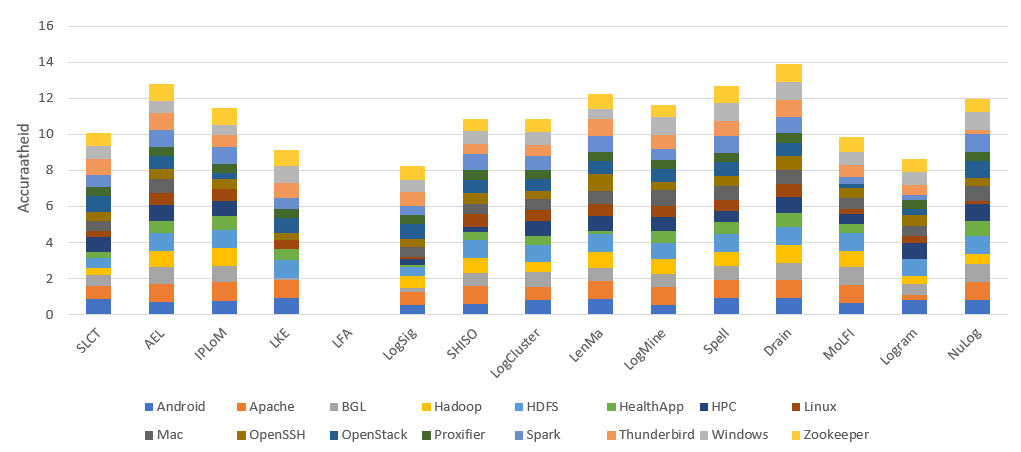
\includegraphics[width=\linewidth]{bp_test_grafiek.png}
    \caption{Weergave van alle parsers in een gestapelde diagram. In de legende worden de kleuren van de verschillende datasets weergegeven.}
    \label{pic:testgrafiek}
\end{figure}

\subsubsection{SLCT}
Bij SLCT is het opmerkelijk dat deze parser vooral aan overfitting doet. Deze parser heeft altijd een zeer laag aantal templates als uitkomst. Bij een inspectie van de templates wordt al snel duidelijk waarom. Deze parser maakt snel gebruik van parameter symbolen waardoor er templates zijn die volledig uit parameters bestaan en op deze manier zijn er honderden lijnen aan gelinkt.\\

Een goed voorbeeld hiervan is de Linux (zie tabel \ref{table:Linux}) dataset. Hierbij kan er gezien worden dat het aantal gewenste clusters gelijk is aan 118, maar SLCT vindt er maar 13.

\subsubsection{AEL}
Deze parser geeft in het algemeen een goed resultaat en werkt op een snel tempo. Op basis van snelheid staat deze parser bijna altijd in de top 3. Bij het bekijken van de accuraatheid wordt het echter duidelijk dat deze parser geen consistente resultaten levert. Zo liggen een deel van de resultaten dichtbij 90 procent maar een even groot deel rond 50 procent. Daardoor geeft figuur \ref{pic:testgrafiek} een vertekend beeld.\\

Deze parser is niet aan te raden omdat deze te onstabiel is tegenover de datasets. Het haalt geen slechte resultaten maar er zijn genoeg andere parsers die beter scoren.

\subsubsection{IPLoM}
Deze parser haalt op veel data sets goeie scores maar bij het onderzoek is gebleken dat deze problemen geeft bij de data set Mac (zie tabel \ref{table:Mac}). De parser loopt vast bij deze dataset ookal zijn dit maar 2000 lijnen. Op de computer gebruikt binnen dit onderzoek kon deze parser niet overweg met deze dataset en dat is reeds een slecht teken wanneer er gezocht wordt naar een parser die met meerdere datasets overweg kan.\\

De resultaten van de andere datasets zijn wel naarbehoren en het is duidelijk dat bij deze datasets de parser goed generaliseert als er gekeken wordt naar de gevonden clusters. Deze gevonden clusters liggen dichtbij het verwachtte resultaat.

\subsubsection{LKE}
Deze parser behaalt geen goede resultaten op vlak van accuraatheid en op vlak van snelheid duurt de parsing meestal langer dan 1 minuut. De snelheid is essentieel binnen dit onderzoek dus een parser die langer dan 1 minuut nodig heeft zal niet tot de conclusie behoren. Neem bijvooerbeeld de scores behaalt op de dataset Hadoop \ref{table:Hadoop}. Hierbij kan waargenomen worden dat de tijd langer is dan 1 minuut en het resultaat is een accuraatheid van 0. Als er dan gekeken wordt naar de gevonden templates dan is het duidelijk dat deze parser problemen had met deze dataset omdat het resultaat maar één cluster bevat dat bestaat uit één enkele parameter.

\subsubsection{LFA} 
Deze parser heeft bij geen enkele dataset een positieve accuraatheid behaalt. De reden wordt duidelijk na een inspectie van de cluster resultaten. Deze bestaan soms uit 1 cluster met niets in of deze zijn zeer specifiek, i.e.\ de cluster lijn is bijna exact hetzelfde als de loglijn. Dit is duidelijk een vorm van underfitting. De parser kan niet goed generaliseren dus zal deze ook niet verder benuttigd worden.

\subsubsection{LogSig}
LogSig behaalt geen goede resultaten op de vergelijkingscriteria. De snelheid is langer dan één seconde, de accuraatheid gaat soms onder 10 procent en de gevonden clusters zijn zeer specifiek. Zo blijven sommige parameternamen perfect behouden en ontstaat er zo een hoop aan gelijkaardige clusters.

\subsubsection{SHISO}
Deze logparser behaalt kleine accuraatheid scores op datasets die veel clusters bevatten. Deze kan duidelijk niet goed generaliseren bij teveel verschillende loglijnen. Zo kan bij het analyseren van de uitkomst voor de Android dataset (zie tabel \ref{table:Android}) gezien worden dat de gevonden clusters nog veel bestandslocaties bevatten die eigenlijk als parameter moeten beschouwd worden.

\subsubsection{LogCluster}
Deze parser had het nadeel dat zelfs met aanpassingen deze niet het aantal clusters wou weergeven die gevonden waren. Hierdoor was dit een moeilijk vergelijkingspunt maar dit hield het onderzoek niet tegen omdat de lage accuratie cijfers reeds genoeg weergeven over de parser en duidelijk maken dat deze niet geschikt is. Als er gekeken wordt naar de resultaten wordt duidelijk waarom deze cijfers zo laag zijn. Veel parameters zoals IP-adressen en poortnummers blijven behouden in de parsing.

\subsubsection{LenMa}
Deze parser behaalt algemeen goeie scores maar geeft bij enkele datasets zoals de Windows dataset (zie tabel \ref{table:Windows}) clusters terug die te specifiek zijn. Dit komt vooral voor bij de langere lijnen. Daardoor komt deze meestal meer clusters uit dan in het resultaat verwacht wordt.\\

Op basis van figuur \ref{pic:testgrafiek} en de resultaten van de parsing lijkt dit een goede parser maar door de lange verwerkings tijden die groter dan één seconde kunnen worden is dit geen parser voor real-time verwerking.

\subsubsection{LogMine}
LogMine geeft meestal wel een goede accuraatheid maar als er gekeken wordt naar de clusters is het duidelijk dat deze zeer generiek kunnen zijn en dus dat de parser aan het overfitten is zoals bij het resultaat van de Android dataset (zie tabel \ref{table:Android}) of dat deze juist zeer specifiek zijn zoals bij het resultaat van de Hadoop dataset (zie tabel \ref{table:Hadoop}).\\

Er zit dus wel een duidelijke fluctatie in de resultaten van deze data set. Hier boven op heeft deze parser ook een zeer lange parsing tijd die meestal boven één seconde gaat.

\subsubsection{Spell}
Spell levert over de verschillende datasets een zeer goed resultaat. Deze parser evenaart bijna Drain in de resultaten. Meestal haalt deze een lagere accuraatheid maar het verschil is zeer klein. Bij het analyseren van de log clusters is het duidelijk dat deze parser meestal goed generaliseert.\\

Er zijn uitzonderingen en als er gekeken wordt naar de Zookeeper dataset (zie tabel \ref{table:Zookeeper}), is het duidelijk dat er veel bestand locaties behouden worden in plaats van deze om te zetten naar parameters maar dit zijn dingen die bij andere parsers ook gebeuren en bij deze parser is dit uitzonderlijk.\\

Omdat deze parser een goed resultaat levert en in totaal vijf keer gemarkeerd staat in de tabellen zal deze verder getest worden door deze te implementeren in LogParse.

\subsubsection{Drain}
Drain was de parser die binnen het vorig onderzoek naar boven kwam als de meest performante parser. Binnen dit onderzoek werd het vorig onderzoek nagebootst maar met aanpassingen dus was het interessant om te zien hoe Drain hieruit ging komen.\\

Binnen dit onderzoek wordt het duidelijk dat Drain nog altijd zeer performant en vooruitstrevend is. Zo kan er uit de tabellen afgeleid worden dat deze parser 10 keer voorkwam tussen de drie beste parsers van een dataset. Dit is veel meer dan elke andere parser dus deze parser zal meegenomen worden naar verder onderzoek met LogParse.\\

De parsings gevonden door Drain zijn meestal gelijkaardig aan de verwachtte parsings en zo behoudt deze parsers een consistente accuraatheid. Als de parsings verder geanaliseerd worden komen hier goede en duidelijke clusters uit. Een uitzondering hierop zijn echter de HealthApp (zie tabel \ref{table:HealthApp}) en OpenStack datasets (zie tabel \ref{table:OpenStack}). Hierbij blijven veel clusters over die hun parameters behouden maar dit is een uitzondering tussen de datasets en hierbij wordt nog een accuraatheid van meer dan 0.7 behouden.

\subsubsection{MoLFI}
Deze parser geeft goede resultaten op papier maar als er gekeken wordt naar de behaalde loglijnen blijkt dat deze parser niet altijd even goede resultaten behaalt. Als het resultaat van de Mac (zie tabel \ref{table:Mac}) of Spark dataset (zie tabel \ref{table:Spark}) bekeken wordt is het duidelijk dat hier geen goede generalisatie plaatsvond en dat dit geresulteerd is in dubbel zoveel patronen dan er verwacht werd. Dit is ook zichtbaar bij OpenStack (zie tabel \ref{table:OpenStack}) maar dit kan goedgepraat worden door het feit dat andere parsers hierbij ook underfitten.\\

Hier boven op heeft deze parser ook veel tijd nodig om de parsing uit te voeren zo worden er soms tijden boven 60 seconden waargenomen.

\subsubsection{Logram}
Deze parser werd toegevoegd aan het rooster binnen dit onderzoek en behaalde op vlak van parsing tijd zeer hoge resultaten. Zo kan er afgeleid worden aan de hand van de tabellen dat deze parser bijna altijd bovenaan staat bij het criterium `Tijd`.\\

De resultaten bij F-Score en Accuraatheid vallen echter tegen. Hierbij haalt de parser meestal slechtere scores dan de oudere parsers en het is duidelijk dat deze eerst nog verder onderzocht moet worden voordat deze een goede parsing voor online streaming zou geven.\\

De gevonden parsings zijn bij de ene helft van de datsets zeer goed en zeer generiek maar bij andere datasets zoals bijvoorbeeld de Apache dataset (zie tabel \ref{table:Apache}) blijven er zeer specifieke clusters over.

\subsubsection{NuLog}
Deze parser werd toegevoegd aan het rooster binnen dit onderzoek en kwam meestal zeer goede resultaten uit. Deze zeer goede resultaten werden meestal behaald door het perfectioneren van de parameters zoals epochs en de grootte van het deel per epoch.\\

Het toepassen van deze parser op nieuwe datasets is echter zeer gecompliceerd. De implementatie van de parser werd verkregen door een repository die hierboven staat vermeld maar hierin zaten maar enkele van de datasets verwerkt. Bij implementatie van de andere datasets werden de resultaten van de parser lager en zelfs bij het aanpassen van de parameters werd dit niet veel beter.\\

Deze parser zou een goede oplossing kunnen bieden voor de onderzoeksvraag maar omdat er nog veel onduidelijkheid is over de inwerking van nieuwe datasets en het aanpassen van de parameters zal het beter zijn om deze verder in de toekomst te gaan onderzoeken.

\subsection{Online vs Offline}
\label{subsection:OnlineOffline}
Wat opvallend is aan de vorige tabellen is dat LogParse nog niet ingerekend staat hierin, dit is omdat LogParse zoals eerder vermeld geen log parser algoritme op zichzelf bezit maar zich baseert op andere parsers en ervoor zorgt dat deze op een efficiëntere en online manier kunnen uitgevoerd worden. Daarom zal hieronder een tabel weergegeven worden van de gekozen log parsers en hun efficiëntie wanneer ze worden ingewerkt in LogParse. Hierbij wordt NuLog overgelaten omdat deze parser niet consistente resultaten weergaf en dus niet geschikt zal zijn voor het antwoord op de onderzoeksvraag.\\

De gekozen logparsers zijn reeds online methodes maar dankzij LogParse kan dit ook effectief getest worden. Door de inwerking in LogParse kan er gekozen worden om een deel van de log lijnen weg te laten en hierdoor kan er op voorand op een trainingsset geparsed worden en deze parsing kan dan getest worden aan de hand van de rest van de log lijnen.\\

De werking met LogParse is wel niet heel eenvoudig en het is moeilijk om nieuwe parsers in te werken omdat hier veel componenten aan vast hangen. LogParse heeft reeds enkele implementatie vrijgegeven in de GitHub repository en hierdoor waren Spell en Drain reeds makkelijk te integreren.\\

Om de werking met LogParse te onderzoeken is er binnen dit onderzoek gekozen om te werken met een trainingsset van 30 procent. Dit betekent dat 70 procent van het log bestand achteraf zal geparsed worden. Om deze configuratie te laten lopen moet er binnen LogParse de volgende commando's uitgevoerd worden:
\begin{verbatim}
    python3 ./splitLog.py -dataset 2kBGL -ratio 0.3 -reprocess True
    python3 ./evaluateLogParse.py -dataset 2kBGL -algorithm Drain
    -choose head -ratio 0.3
\end{verbatim}
Merk hierbij op dat de ratio variabele de grootte van de trainingsset weergeeft. Na deze commando's kan de rest van de dataset geëvalueerd worden met het volgend commando:
\begin{verbatim}
    python3 ./logTIM.py Drain 2kBGL 0.3 1
\end{verbatim}

Hierdoor zal een evaluatie van de log parser gemaakt worden. In de tabel hieronder wordt een weergave gegeven van de evaluatie met LogParse in vergelijking met de offline manier. Hierbij wordt enkel gekeken naar de tijd, f-score en het aantal gevonden clusters.

In tabel \ref{table:onlinetabel} wordt weergegeven dat de parsers duidelijk minder goede resultaten behalen. Accuraatheid is moeilijk te vergelijken omdat dit niet in de LogParse code ingewerkt kon worden maar dankzij de f-score en het aantal clusters kan er reeds een duidelijk verschil waargenomen worden.

\begin{table}[!htp]
    \caption{Tabel met vergelijking van offline vs online behaalde scores van de gekozen log parsers met toepassing op de fractionele data set BGL.}
    \label{table:onlinetabel}
    \begin{center}
        \begin{tabular}{||c | c | c | c||} 
            \hline
            Parser & Tijd & F-Score & Aantal clusters \\ [0.5ex] 
            \hline\hline
            
            Spell & 0.64s & 0.9569 & 262 \\
            
            Spell Online & 0.86s & 0.3992 & 54 \\
            
            Drain & 0.44s & 0.9996 & 108 \\
            
            Drain Online & 0.85s & 0.6914 & 72 \\

            \hline
        \end{tabular}
    \end{center}
\end{table}

\subsection{Nieuwe datasets}
In deze laatste sectie is het de bedoeling om de gekozen parsers, i.e.\ Drain, NuLog en Spell onderhevig te stellen aan nieuwe datasets en de resultaten te analyseren. Deze datasets waren veel groter dan de vorige datasets en dit was merkbaar in de parsing tijd.\\

Hierbij is er begonnen met de dataset verkregen via de co-promotor van deze bachelorproef. Deze dataset heet `alert\_Orval` en hieronder staat een representatie van de lijnen binnen deze dataset:
\begin{verbatim}
    2019-06-08T08:39:32.993572+00:00
    DBW0 started with pid=26, OS id=39223 
    Starting background process CKPT
    2019-06-08T08:39:33.047980+00:00
    LGWR started with pid=27, OS id=39227 
    2019-06-08T08:39:33.118417+00:00
    CKPT started with pid=28, OS id=39231 
    2019-06-08T08:39:33.225755+00:00
    LGWR slave LG00 created with pid=29, OS pid=39235
    Starting background process SMON
\end{verbatim}
Hieruit is een patroon af te leiden dat begint met de datum, dan het uur en uiteindelijk op een nieuwe lijn het event. Dit patroon was moeilijk in te werken binnen dit onderzoek omdat deze parsers lijn per lijn lopen. Als gevolg gaven de parsers voor deze dataset geen goede resultaten terug. De tijd die het de parsers nam om deze dataset te verwerken was bij Drain wel veelbelovend. Zo duurde het maar 15.8 seconden voor Drain om deze dataset van 50000 lijnen te parsen met een gemiddelde van 0.41 seconden op 2000 lijnen is dit een zo goed als lineaire ontwikkeling. Bij Spell duurde dit maar liefst 78.2 seconden en bij NuLog was dit onmogelijk weer te geven omdat de opzet van het model te lang duurde.\\

Om toch een beter overzicht te krijgen over de invloed van een nieuwe dataset op deze parsers is er een tweede dataset gekozen die online verkrijgbaar was op Kaggle.com \footnote{https://www.kaggle.com/shawon10/web-log-dataset}. Deze dataset heet de web log dataset en geeft enkele loglijnen die verschillende http aanvragen bevat. Hieronder worden enkele lijnen van deze dataset weergegeven:
\begin{verbatim}
    10.131.2.1,[29/Nov/2017:06:59:37,GET /logout.php HTTP/1.1,302
    10.131.2.1,[29/Nov/2017:06:59:37,GET /login.php HTTP/1.1,200
    10.130.2.1,[29/Nov/2017:07:00:19,GET /login.php HTTP/1.1,200
    10.130.2.1,[29/Nov/2017:07:00:21,GET /login.php HTTP/1.1,200
\end{verbatim}
Deze blijven wel op één lijn en er is een duidelijk patroon per lijn zichtbaar namelijk IP-adress, datum, tijd, soort request en het resultaat. Dit is omgezet naar het volgend log formaat binnen de parsers:
\begin{verbatim}
    <IP>,\[<Date>:<Time>,<Content>,<Result>
\end{verbatim}

Drain heeft deze logfile van 16000 lijnen verwerkt in 2.22 seconden en gaf hierbij een zeer goede representatie van de lijnen met een totaal van 5 verschillende clusters die correspondeerden met de methode namen zoals `GET`, `POST`, etc.. Hieronder wordt de uitkomst van Drain weergegeven:
\begin{verbatim}
    EventId,EventTemplate,Occurrences
    164340f3,GET <*> HTTP/1.1,15054
    c9d30e53,POST <*> HTTP/1.1,679
    7a4315b8,GET <*> HTTP/1.0,44
    2f89ed1b,HEAD <*> HTTP/1.1,9
    cfadd2fa,POST <*> HTTP/1.0,3
\end{verbatim}

NuLog duurde langer om te runnen door het opstellen van het model maar gaf als uitkomst clusters die door elkaar lopen. Om alle clusters te achterhalen zou deze parser uitgebreid moeten worden met een cluster weergave zoals de andere parsers. Uit de logs zelf kan echter geconstateerd worden dat de parser nog zeer specifiek blijft en veel parameters zoals css bestandslocaties heeft overgelaten. Hieronder wordt en deel van ede uitkomst van NuLog weergegeven:
\begin{verbatim}
    ac6cccffea9df8ef06deb8200bbaba5b,GET /css/bootstrap.min.css <*>
    4264885f9e74401dafa7b41a326deb37,GET /css/font-awesome.min.css <*>
    3f7c955e48a2c50bfc49e2c861a8edc1,GET /css/normalize.css <*>
    bb1e3aa06724c3a7a34430129685687b,GET /css/main.css <*>
    7b82aabfa0dc9640b47712a4ac047b71,GET /css/style.css <*>
    c3ca126691345d5ca34d7f5efcb0f219,GET <*> <*>
    c3ca126691345d5ca34d7f5efcb0f219,GET <*> <*>
\end{verbatim}

Spell heeft deze logfile op 2.21 seconden tijd maar was hierbij aan het underfitten en gaf veel te specifieke clusters waardoor er uiteindelijk 121 verschillende clusters aanwezig waren in de oplossing. Hieronder wordt een deel van de uitkomst van Spell weergegeven.:
\begin{verbatim}
EventId,EventTemplate,Occurrences
7034a1ef,GET /login.php HTTP/1.1,3284
38076aba,POST /process.php HTTP/1.1,312
cc86797f,GET /home.php HTTP/1.1,2640
8df1ed4b,GET /js/vendor/moment.min.js HTTP/1.1,173
615bad2c,GET /bootstrap-3.3.7/js/bootstrap.js HTTP/1.1,191
75a6659a,GET <*> bala HTTP/1.1,2
dcb2622d,GET /js/jquery.min.js HTTP/1.1,56
\end{verbatim}